\appendix
\appendixpage

\chapter*{Contexte de l'open source}

\begin{figure}[ht]
	\center
	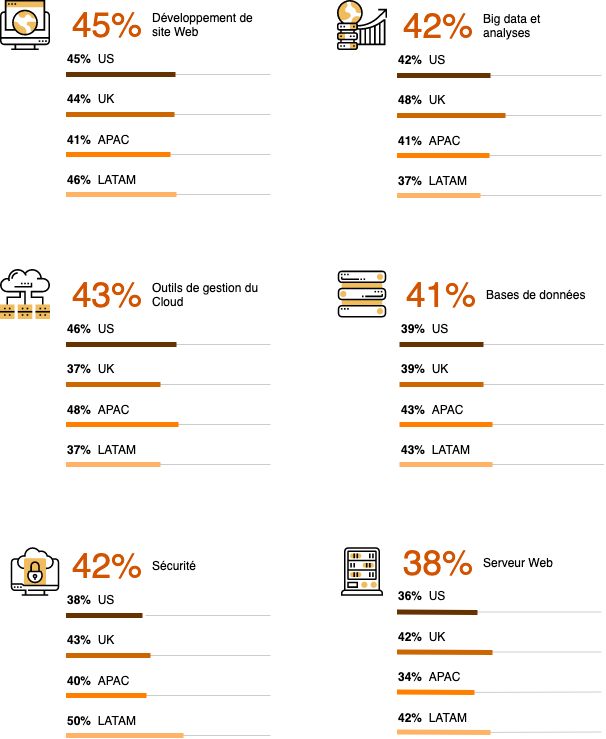
\includegraphics[scale=0.65]{./img/Domain_os.png}
	\caption{Domaine d'application de l'open source dans l'IT}							
	\caption*{\color{silver}Source: redhat.com}					
\end{figure}

\begin{figure}[ht]
	\center
	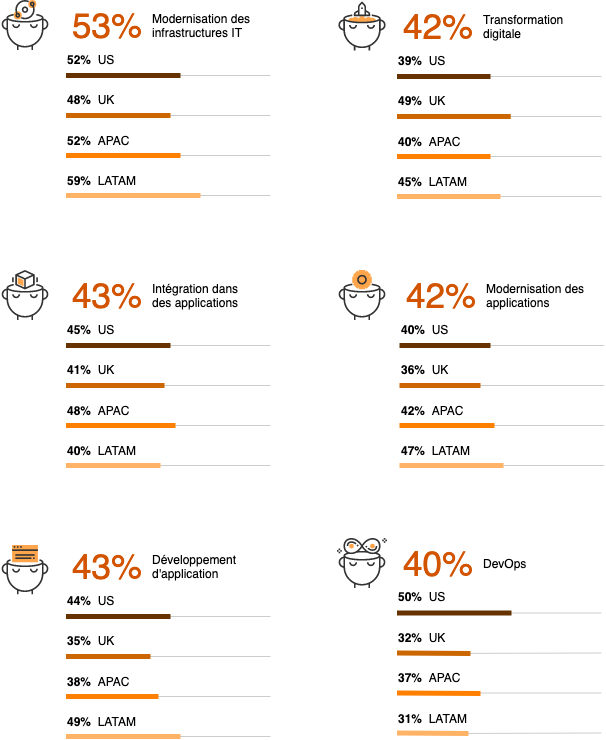
\includegraphics[scale=0.65]{./img/Use_os.png}
	\caption{Secteur d'application de l'open source}
	\caption*{\color{silver}Source: redhat.com}					
\end{figure}

\chapter*{Formulaire}

	\begin{figure}[ht]
		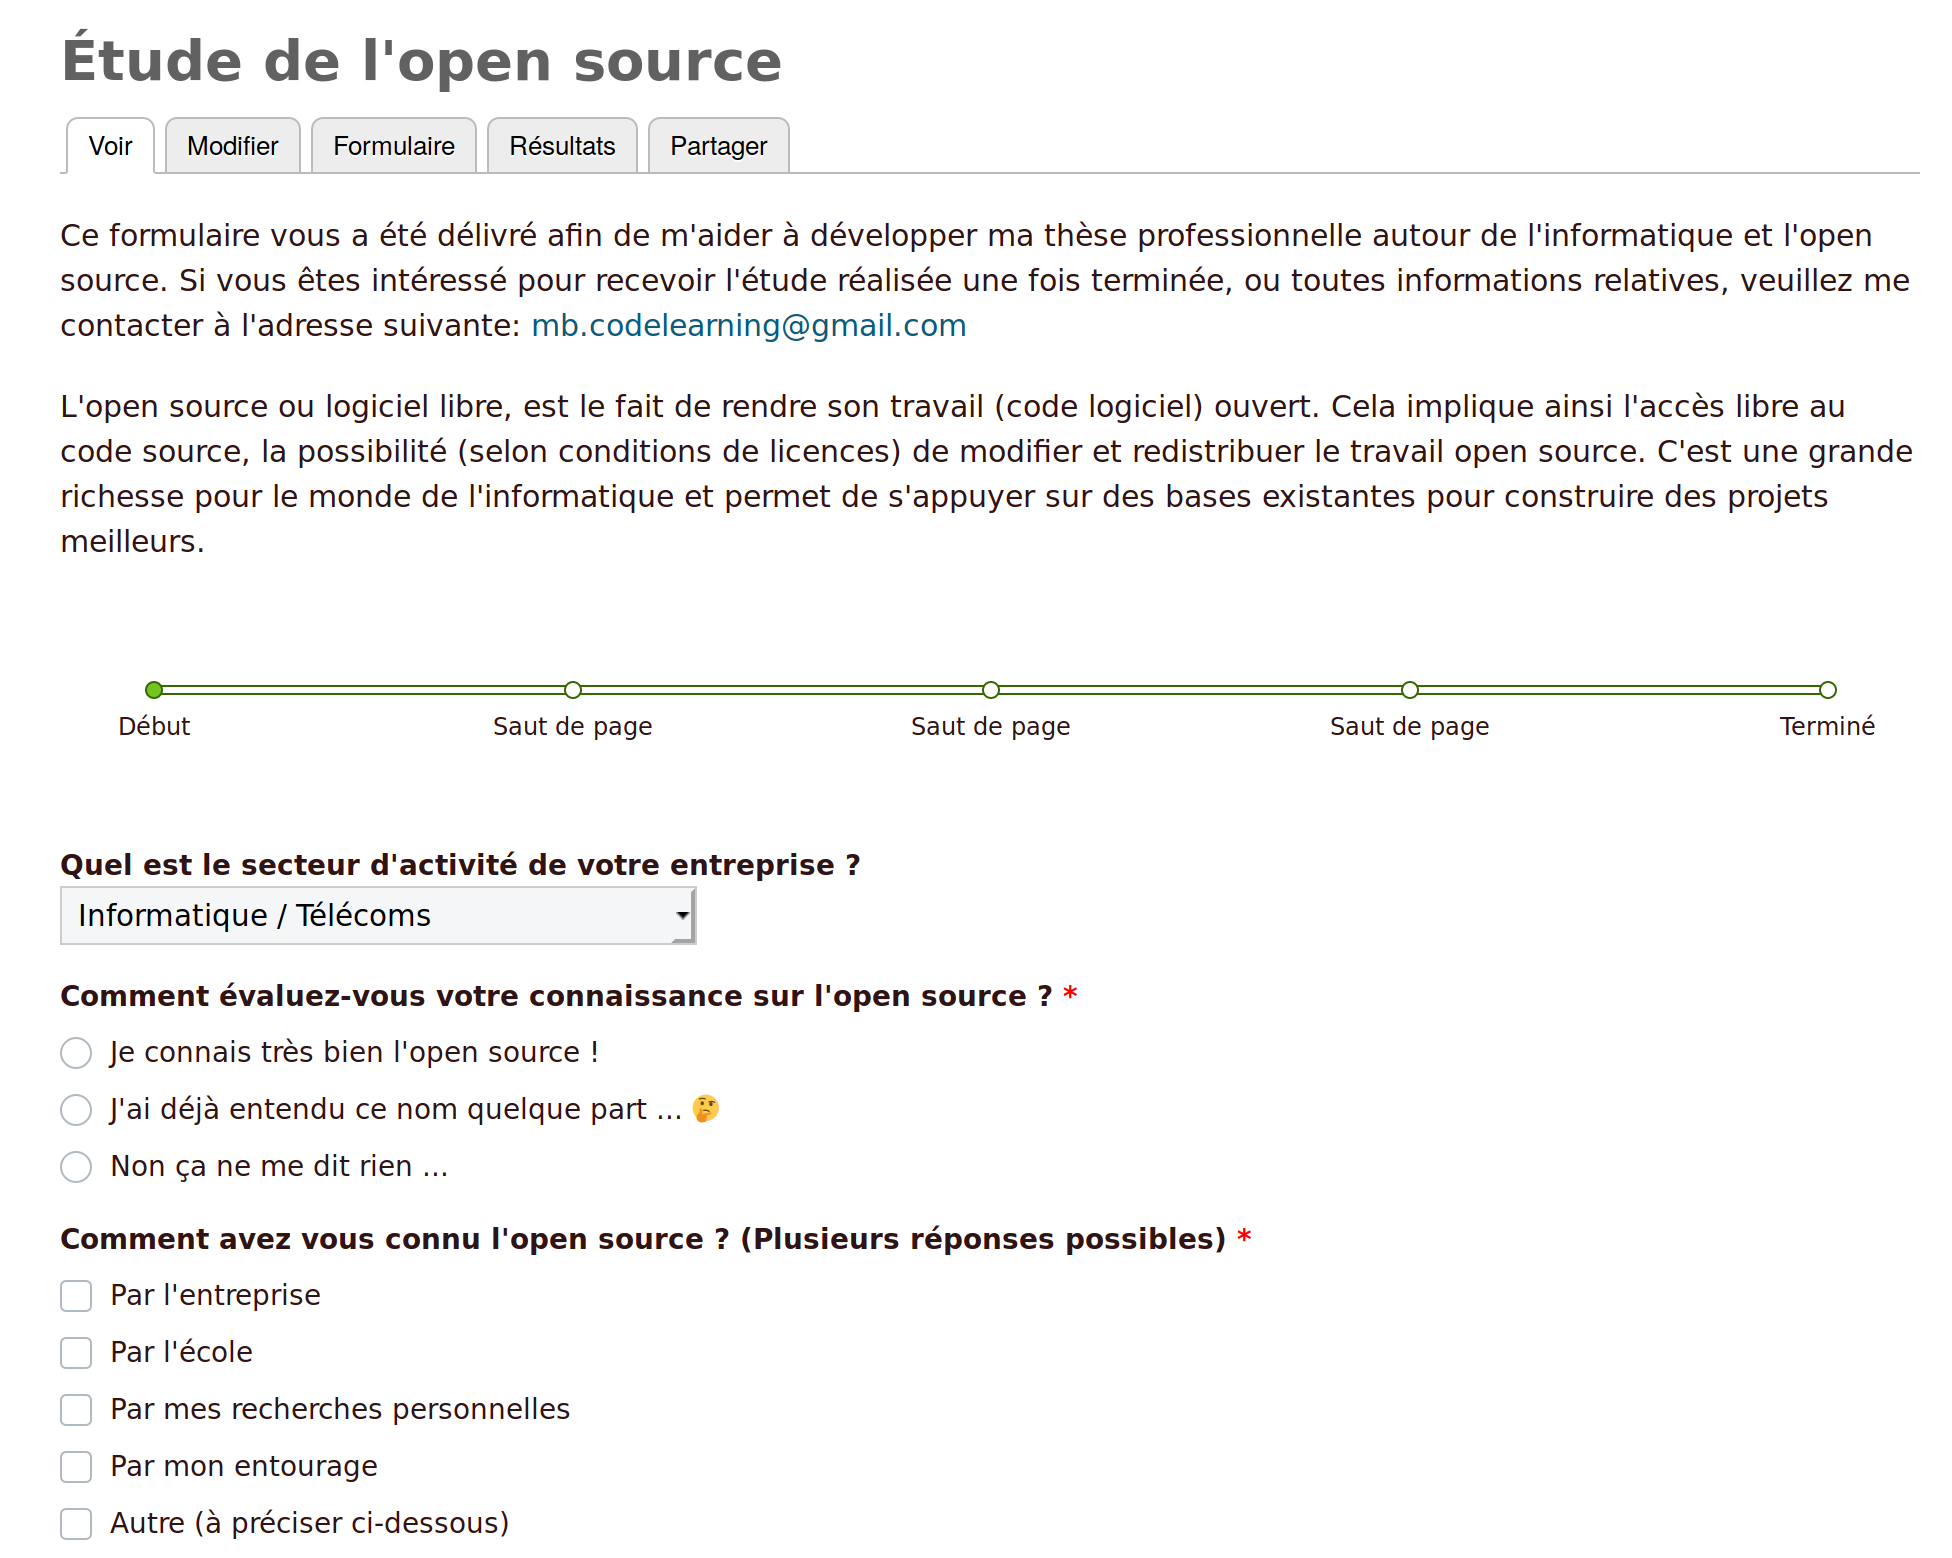
\includegraphics[scale=0.25]{./img/f1.png}
		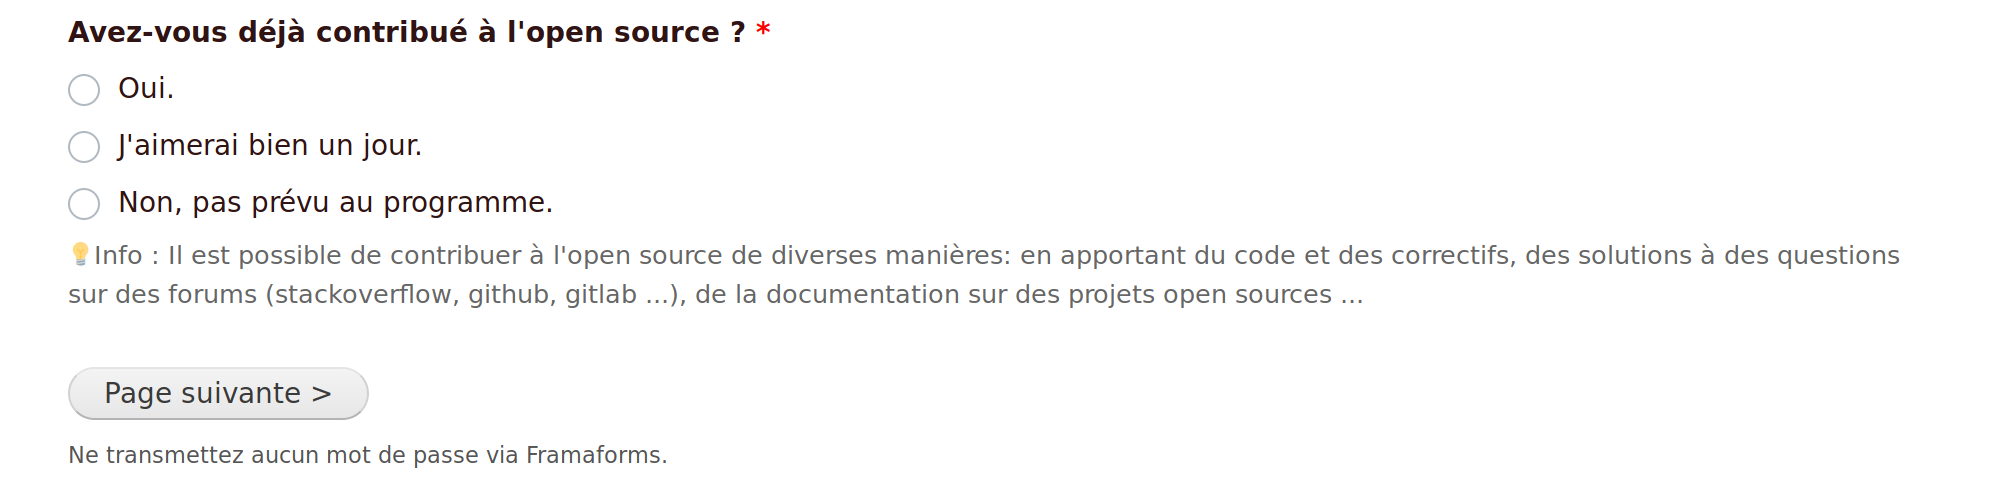
\includegraphics[scale=0.25]{./img/f2.png}
	\end{figure}
	\begin{figure}[t]
		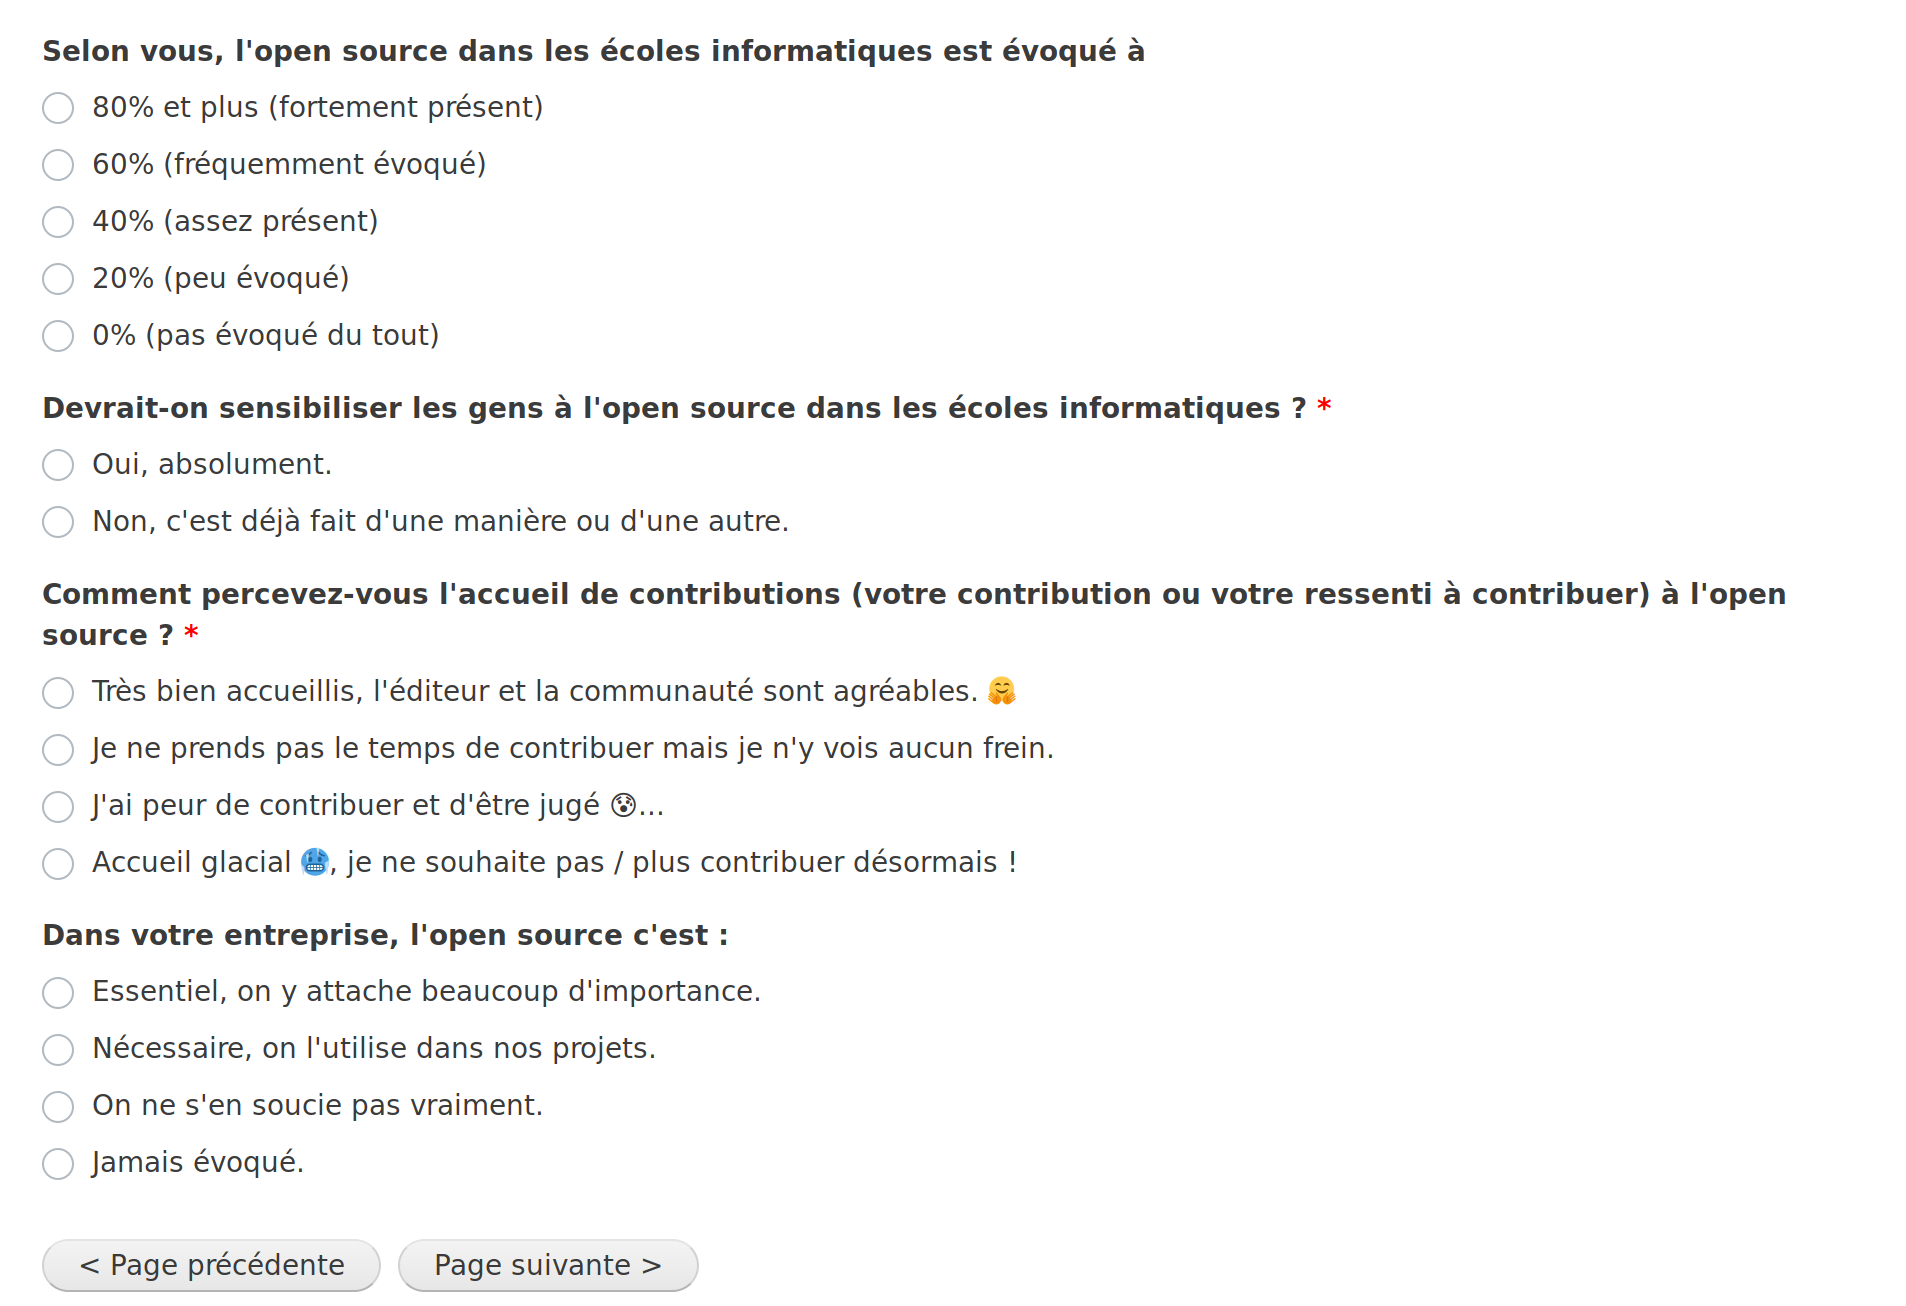
\includegraphics[scale=0.25]{./img/f3.png}
		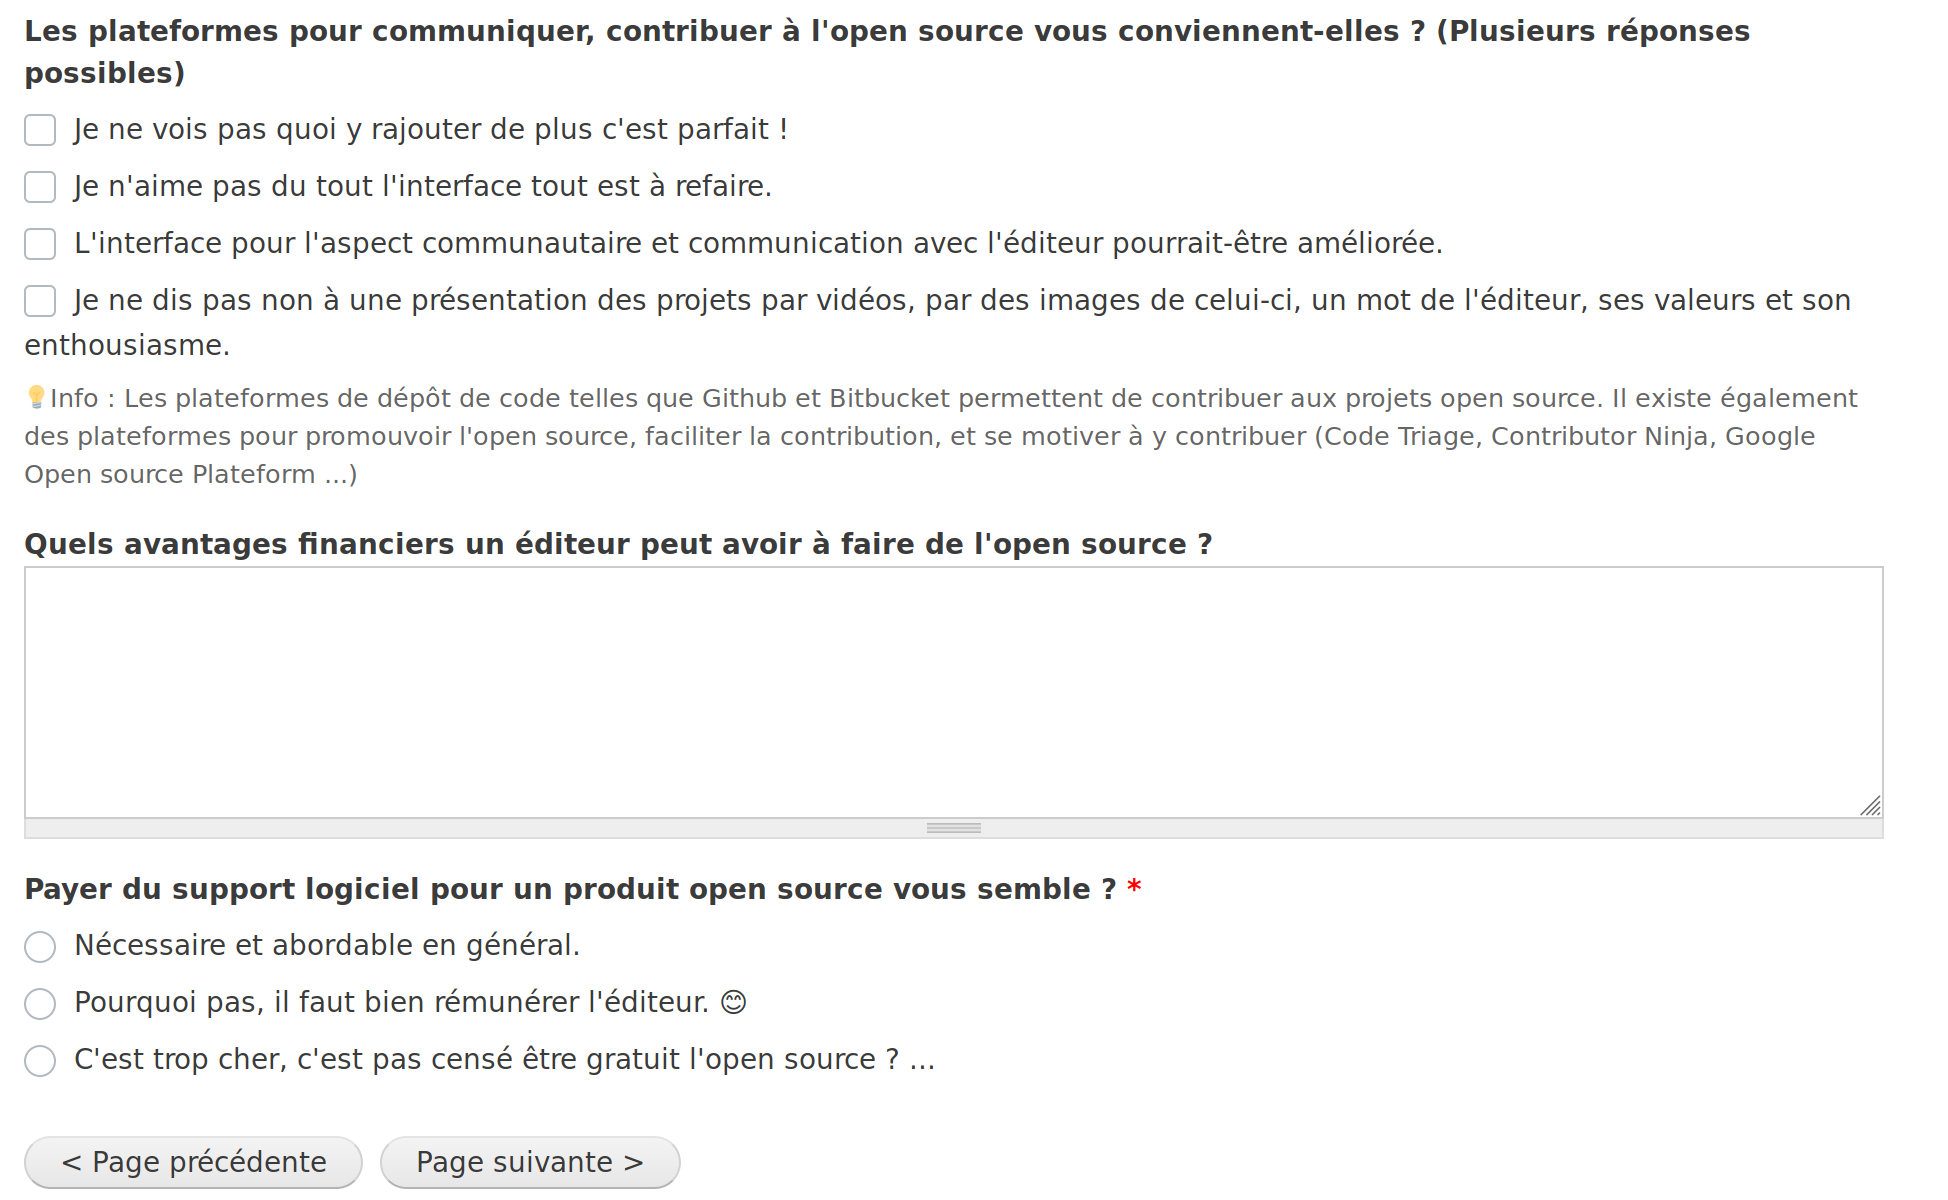
\includegraphics[scale=0.25]{./img/f4.png}
	\end{figure}	
	\begin{figure}[t]
		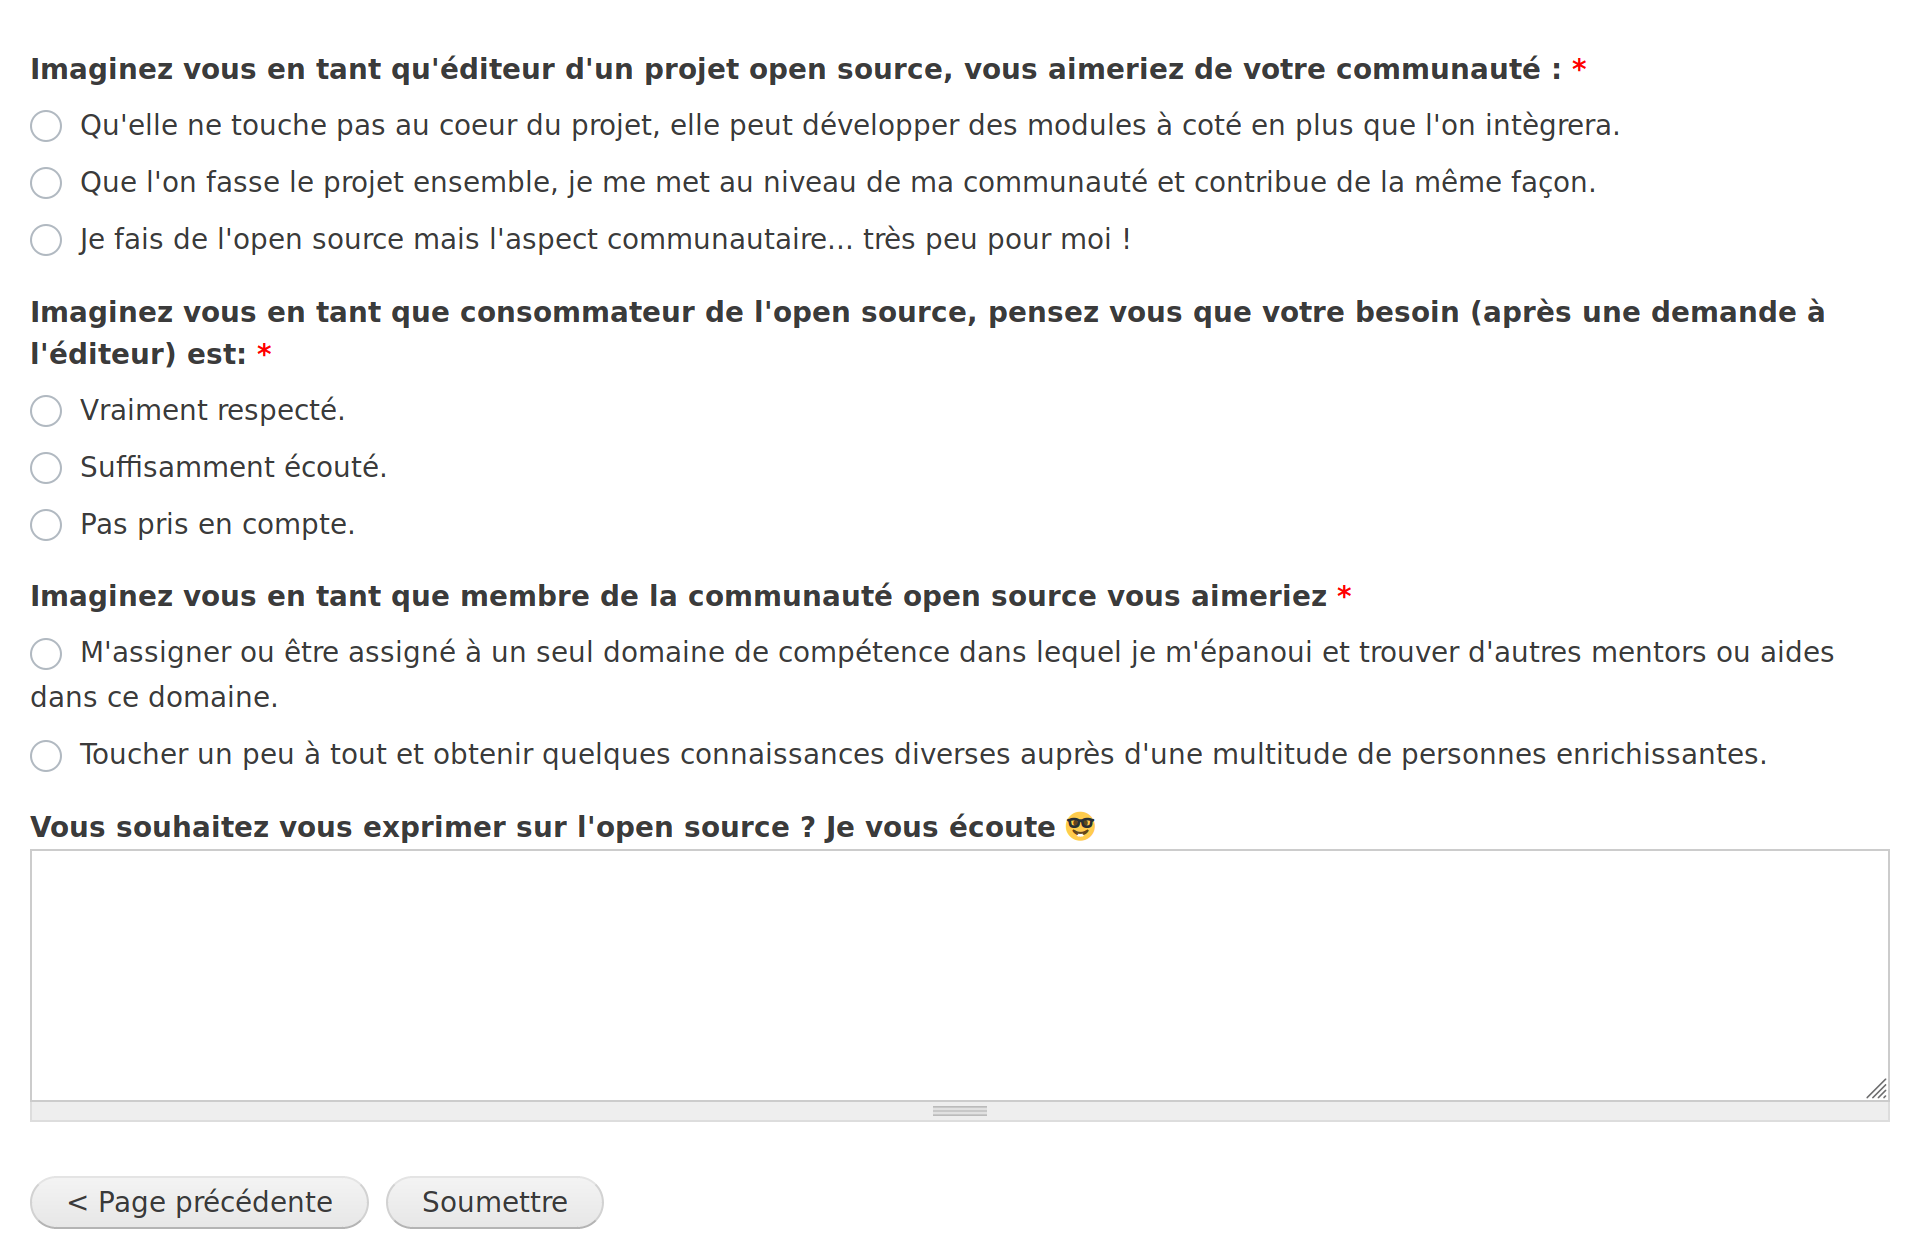
\includegraphics[scale=0.25]{./img/f5.png}
	\end{figure}	
\chapter*{Interview}

\section*{Plateformes promotrices}

\begin{itemize}[label=\textbullet, font=\LARGE \color{burntorange}]
	\item Que pensez-vous des plateformes actuelles qui promouvoient l'open source ?\\
	\hbox to 15cm{\leaders\hbox to 10pt{\hss . \hss}\hfil}
	\item Trouvez vous l'interface, pratique, ludique et acueillante pour vous, votre recherche, et vos contributions éventuelles ?\\
	\hbox to 15cm{\leaders\hbox to 10pt{\hss . \hss}\hfil}
	\item Y-voyez vous un frein à ce que les consommateurs de l'open source, participent, recherchent et utilisent l'open source.\\
	\hbox to 15cm{\leaders\hbox to 10pt{\hss . \hss}\hfil}
	\item Si vous deviez améliorer une chose à la plateforme que vous utilisez pour trouver de l'open source, quelle serait-elle ?\\
	\hbox to 15cm{\leaders\hbox to 10pt{\hss . \hss}\hfil}

\end{itemize}

\section*{Gestion des ressources}

\begin{itemize}[label=\textbullet, font=\LARGE \color{burntorange}]
	\item Comment trouvez vous la gestion de la communauté open source ?\\
	\hbox to 15cm{\leaders\hbox to 10pt{\hss . \hss}\hfil}
	\item Actuellement le mode de management des projet open source est de développer le coeur du projet pour l'éditeur et de rajouter des extensions (si accepté) développées par la communauté. Qu'en pensez-vous ?\\
	\hbox to 15cm{\leaders\hbox to 10pt{\hss . \hss}\hfil}
	\item La relation hiérarchique et les échanges vous convient-elle ?\\
	\hbox to 15cm{\leaders\hbox to 10pt{\hss . \hss}\hfil}
	\item Si vous développez pour l'open source, préferreriez vous toucher à tout dans le projet ou plutot être assigné à une zone de compétence spécifique ?\\
	\hbox to 15cm{\leaders\hbox to 10pt{\hss . \hss}\hfil}
	\item La multi-compétences (faire un peu de front, du back, du design, et de la base de données) est-elle une perte d'efficacité ou un gain à vos yeux ?\\
	\hbox to 15cm{\leaders\hbox to 10pt{\hss . \hss}\hfil}
	\item Si vous connaissiez la but final de l'éditeur et de son projet open source, ses valeurs,et que celles-ci correspondent à votre vision, celà vous donnerai-il plus envie de contribuer à ce projet\\
	\hbox to 15cm{\leaders\hbox to 10pt{\hss . \hss}\hfil}
\end{itemize}

\newpage
\section*{Chez le consommateur}

\begin{itemize}[label=\textbullet, font=\LARGE \color{burntorange}]
	\item Selon-vous, qui est consommateur de l'open source ?\\
	\hbox to 15cm{\leaders\hbox to 10pt{\hss . \hss}\hfil}
	\item Pensez vous que les échanges (demandes, commentaires) avec les utilisateurs de l'open source sont bien accueillis ?\\
	\hbox to 15cm{\leaders\hbox to 10pt{\hss . \hss}\hfil}
	\item Faut-il sensibiliser le consommateur (entreprise numérique ou particulier) à l'open source ?\\
	\hbox to 15cm{\leaders\hbox to 10pt{\hss . \hss}\hfil}
	\item Je trouve que le milieu scolaire ne m'a pas assez sensibilisé à l'importance de l'open source, quel est votre avis ?\\
	\hbox to 15cm{\leaders\hbox to 10pt{\hss . \hss}\hfil}
\end{itemize}

\section*{Marketing de l'open source}

\begin{itemize}[label=\textbullet, font=\LARGE \color{burntorange}]
	\item Si vous développiez un projet open source, que feriez vous pour attirer le consommateur ?\\
	\hbox to 15cm{\leaders\hbox to 10pt{\hss . \hss}\hfil}
	\item Faut il améliorer le marketing sur les plateformes qui promouvoie l'open source ?\\
	\hbox to 15cm{\leaders\hbox to 10pt{\hss . \hss}\hfil}
	\item Je pensais à utiliser un système de présentation de projet, une vidéo comme un kickstarter pour adhérer au projet, ses missions, et valeurs ainsi qu'une page de présentation ? Est-ce une bonne idée selon vous ?\\
	\hbox to 15cm{\leaders\hbox to 10pt{\hss . \hss}\hfil}
	\item Comment pensez vous que l'open source attire le consommateur ?\\
	\hbox to 15cm{\leaders\hbox to 10pt{\hss . \hss}\hfil}
	\item Est-ce que vous déploierait des moyens publicitaires (campagnes, pancartes, évènements, ...) pour promouvoir votre projet Open source ou seul le projet et son hébérgement suffit?\\
	\hbox to 15cm{\leaders\hbox to 10pt{\hss . \hss}\hfil}
\end{itemize}